\chapter{Lists}

Natural numbers constitute an important example of something more
general, where objects are built up from simpler
ones. The Axiom of Induction captures the idea of building ``up''
and provides an important method for proving facts about natural
numbers.

In this lecture, we develop an analogous way to think about \emph{lists}. 

\begin{goals}
\noindent \textbf{Lecture Goals}
\begin{itemize}
\item Introduce a formal counterpart to the informal concept of a list
\item Emphasize the close analogy between lists and natural numbers
\item Introduce basic operations on lists.
\end{itemize}

\noindent\textbf{Study Goals}
\begin{itemize}
\item Demonstrate facility with basic list manipulation including calculating length and 
concatenation of lists.
\end{itemize}
\end{goals}

\section{Lists}

\ignore{
For natural numbers $0$ and $n^\nxt$ are the only ways to construct
natural numbers. Operations like addition and multiplication are
defined in terms of $0$ and ${}^\nxt$, so they do not contribute directly
to the \emph{construction} of natural numbers.

We refer to $0$ and $\nxt$ as \emph{constructors}.  Axioms
\ref{ax:NatZero} and \ref{ax:NatPred} spell out how these
constructors behave.  Axiom \ref{ax:NatZero} captures the idea that
each constructor is entirely different from the other: $0\neq n^\nxt$.
Axiom \ref{ax:NatPred} captures the idea that ${}^\nxt$ constructs
distinct natural numbers from distinct natural numbers: $m^\nxt =
n^\nxt$ implies $m=n$.

So the basic ingredients of natural numbers are the constructors $0$
and ${}^\nxt$ with the understanding that (a) they each produce
different results and (b) from different ingredients, ${}^\nxt$
produces different results. In fact, point (b) also applies to $0$
trivially, because $0$ does not use any ingredients.

We can summarize everything we want to say about natural numbers
concisely in the following way.

\begin{definition}
  The \emph{natural numbers} are defined \emph{inductively} by
  \begin{align*}
    n &\defeq 0 \mathrel{\mid} n^\nxt
  \end{align*}
\end{definition}

In this notation, the vertical bar separates the different constructors for
natural numbers.  The first constructor ($0$) does not depend on
anything else. The second constructor depends on a natural number $n$
and produces a new one $n^\nxt$. So this gives a very concise description of the signature of natural numbers.
Implicitly, this notation is meant to
indicate that the two alternatives are completely distinct. This is
Axiom \ref{ax:NatZero}.  Also implicitly, ${}^\nxt$ is meant to produce
distinct results from distinct $n$'s.  This is Axiom
\ref{ax:NatPred}.  By saying that this defines natural numbers
\emph{inductively}, we also implicitly include the Axiom of
Induction. Namely, no natural numbers can be removed without violating
the structure.

Other kinds of mathematical objects can be defined by inductively by
describing their construction. Indeed, many important types of data in computing
are defined inductively. 
}

In this section, we concentrate on the fundamental concept of \emph{lists}. The idea is really meant to
be the familiar one, so a list of ``to do'' items is a list. The alphabetized names on a class roster is a list. 
We will write lists using square brackets. So for example, $[2,3,5,7]$ is the list of 
the prime numbers less than $10$ in ascending order. For lists, we expect the order to matter. 
So $[7,5,3,2]$ is a different list.

Something that occurs on a list is called an \emph{item} of the list. We can even
specify where it is. So we can talk about the ``first'', ``second'' item, and so on, 
assuming the list has enough items. 

Because we have already agreed that natural numbers begin with $0$, it turns out to make
many things easier if we change the way we talk about items on a list to gibe with the natural
numbers. So instead of refering to the ``first'' item, we might call it the ``initial'' item.
Furthermore, we will number them to start with $0$. What I mean is that if $L=[2,3,5,7]$,
we will write $L_0$, $L_1$, $L_2$, $L_3$ for the elements $2$, $3$, $5$, $7$, respectively. 
In short, the ``initial'' item is indexed by the ``initial'' natural number $0$. The next item after that is indexed by next natural number, $0^\nxt$,
and so on.

Like natural numbers, lists can be built up by starting with an empty list and incrementally adding items. We have choices 
for how we might formalize the idea. We will follow a standard that has developed in computer science. Clearly, since we use 
square brackets to punctuate lists, the empty list should be written as $[\,]$. To add an item to a list, we will conventionally
put it on the front.  

Given the list $[x,y,z]$, we may build a new list with initial item $w$ and the given list as the rest, resulting in $[w,x,y,z]$.
The operation of \emph{prepending} an item to a list is denoted by a colon (:). 
So $w:[x,y,z]$ \emph{is} the list $[w,x,y,z]$.

The empty list, together with prepending items, gives us a way to construct any list we want.

\ipadbreak

\begin{example}
  Here are some examples.
  \begin{itemize}
  \item $5:6:[4,5]$ is the same as $5:[6,4,5]$, which is the same as
    $[5,6,4,5]$.
  \item $[\,]$ is the empty list
  \item $1:[\,]$ is the same as $[1]$
  \item $1:2:3:4:[\,]$ is the same as $[1,2,3,4]$.
  \end{itemize}
\end{example}

Notice that every list is either empty ($[\,]$) or not. If not, it has
the form $x:L$ where $x$ is the initial item and $L$
is the rest of the list. This suggests a signature for lists, not so different from
the signature for natural numbers.

\begin{signature}{sig:list}
	Lists have the following basic structure.
	  \begin{itemize}
	  \item There is a special list, which we call \emph{the empty list} and denote by $[\,]$.
	  \item For any thing $x$ and any list $L$, there is another list, obtained by \emph{prepending} $x$ to $L$. We denote
	  the result by $x:L$.
	  \end{itemize}
\end{signature}

As with the natural numbers, we need to think about axioms that prevent strange behavior. These are exactly analogous to the
axioms of natural numbers. First, $[\,]$ can not be obtained by adding a new initial item to another list. So

\begin{axiom}
	For any list $L$ and any thing $x$, $[\,]\neq x:L$.
\end{axiom}

Likewise, a list that is not empty can only be built one way.

\begin{axiom}
	For any things $x$ and $y$ and lists $L$ and $M$, if $x:L = y:M$, then $x=y$ and $L=M$.
\end{axiom}

For example, if I tell you that $[2,3,4,5] = x:L$, then you know immediately that $x=2$ and $L=[3,4,5]$.

Finally, lists need an induction axiom that ensures that all lists are built up from $[\,]$.


\begin{axiom}\label{ax:NatInd}
	[The Axiom of List Induction] No lists can be removed without violating \ref{sig:list}.
\end{axiom}

This axiom justifies conducting proofs about all lists by a scheme almost identical to simple arithmetic induction.
That is, to prove some property is true about all lists, it is enough to show
\begin{itemize}
\item{}[Basis] The property is true about $[\,]$.
\item{}[Inductive Hypothesis] Assume that the property is true for from list $K$.
\item{}[Inductive Step] Prove that for any thing $x$, the property is true about $x:K$. [You may use the
  assumption about $K$ in this part of the proof.]
\end{itemize}

Operations on lists can now also be defined by schemes similar to how 
we defined addition and multiplication on natural numbers. For example,
every list has a length. Writing $\len(L)$ for the length of a list,
$\len([2,3,4]) = 3$.  A precise definition is now easy to formulate.

\begin{definition}
  For a list $L$. the \emph{length} of $L$, denoted by $\len(L)$, is
  the natural number. This satisfies the following equalities.
  \begin{align*}
    \len([\,]) &= 0\\
    \len(x:L) &= len(L)^\nxt
  \end{align*}
\end{definition}

\begin{example}
  \begin{align*}
    \len([2,3,4]) &= \len(2:[3,4])\\
    &= \len([3,4])^\nxt\\
    &= \len(3:[4])^\nxt\\
    &= \len([4])^{\nxt\nxt}\\
    &= \len(4:[\,])^{\nxt\nxt}\\
    &= \len(,])^{\nxt\nxt\nxt}\\
    &= 0^{\nxt\nxt\nxt}\\
    &= 3
  \end{align*}
\end{example}

\ipadbreak

Another common operation on lists is \emph{concatenation}:
$[2,3,4]\otimes[4,1,3] = [2,3,4,4,1,3]$, whereby the two lists are simply glued together in their original orders.  This is defined precisely by
the following.

\begin{defn}
  For lists $L$ and $M$, their \emph{concatenation}, denoted by
  $L\otimes M$, is a list. For all lists $M$, the following are true.
  \begin{align*}
    [\,]\otimes M &= M\\
    (x:K)\otimes M &= x:(K\otimes M) & \text{for any thing $x$ and any list $K$}
  \end{align*}
\end{defn}

\begin{example}
  To calculate $[4,5,2,1] \otimes [3,4,1]$, we can follow a method similar to arithmetic:
  \begin{align*}
    [4,5,2,1]\otimes[3,4,1] &= (4:5:2:1:[\,])\otimes[3,4,1] & \text{[$[4,5,2,1]$ abbreviates $4:5:2:1:[\,]$]}\\
                    &= 4:((5:2:1:[\,])\otimes[3,4,1]) &\text{[Def. of $\otimes$]}\\
                    &= 4:5:((2:1:[\,])\otimes[3,4,1]) & \text{[Same]}\\
                    &= 4:5:2:((1:[\,])\otimes[3,4,1]) &\text{[Same]}\\
                    &= 4:5:2:1:([\,]\otimes[3,4,1])  &\text{[Same]}\\
                    &= 4:5:2:1:[3,4,1] &\text{[Same]}\\
                    &= [4,5,2,1,3,4,1]                &\text{[Abbreviation]}
  \end{align*}
\end{example}

\ipadbreak
Now we can prove some useful facts about lists.

\begin{lemma}
  On lists, $[\,]$ is the identity for $\otimes$,

\begin{proof}
  By definition
  $[\,]\otimes L = L$ always true.  But $[\,]$ must also 
  satisfy
  $L\otimes[\,] = L$ always. We can proceed by
  induction on $L$. The proof should look familiar (see the proof of
  Lemma \ref{lem:AddZero}).

  \begin{itemize}
  \item{}[Basis] $[\,]\otimes [\,] = [\,]$ is true by definition of
    $\otimes$.
  \item{}[Inductive Hypothesis] Assume $K\otimes[\,] = K$ for some list
    $K$.
  \item{}[Inductive Step]  Suppose $x$ is some thing. We need to show that $(x:K) \otimes [\,] = x:K$. 
    \begin{align*}
       (x:K)\otimes [,\] &= x:(K\otimes[\,]) &\text{[by definition of $\otimes$]}\\
	                   &= x:K &\text{[by the Inductive Hypothesis]}   	
    \end{align*}
  \end{itemize}
  Thus (by the Axiom of List Induction), the lists for which $L\otimes [\,] = L$ constitute all lists.
\end{proof}
\end{lemma}


\ipadbreak

\begin{lemma}
On lists, $\otimes$ is associative.

\begin{proof}
We prove $L\otimes(M\otimes N) =
  (L\otimes M)\otimes N$ using induction on $L$. This should look
  familiar. It is almost identicial to the proofs that addition and
  multiplication are associative.

  \begin{itemize}
  \item{}[Basis] $[\,]\otimes(M\otimes N) = M\otimes N = ([\,]\otimes M)\otimes
    N$. Both steps are by the definition of $\otimes$.
  \item{} [Inductive hypothesis] Suppose $K\otimes(M\otimes N) = (K\otimes
    M)\otimes N$ for some particular list $K$.
  \item{} [Inductive step]
    \begin{align*}
      (x:K)\otimes (M\otimes N) &= x:(K\otimes (M\otimes N)) &\mbox{Def. of $\otimes$}\\
      &= x:((K\otimes M)\otimes N) &\mbox{Inductive Hypothesis}\\
      &= (x:(K\otimes M))\otimes N &\mbox{Def. of $\otimes$}\\
      &= ((x:K)\otimes M)\otimes N &\mbox{Def. of $\otimes$}
    \end{align*}
  \end{itemize}
  So $L\otimes(M\otimes N) = (L\otimes M)\otimes N$ is true for all $L$. Since the proof
  does not depend on any special propertis of $M$ and $N$ (except that they are both lists),
  the result is true for all lists $M$ and $N$.
\end{proof}
\end{lemma}

\ipadbreak

Here is another nice fact that we can prove by induction relating
length to concatenation.

\begin{lemma}
  For any lists $L$ and $M$, $\len(L\otimes M) = \len(L)+\len(M)$.

\begin{proof} [This claim is probably fairly obvious to
  you. Nevertheless, to illustrate the technique of list
  induction again, we prove it explicitly.]
  \begin{itemize}
  \item {}[Basis] $\len([\,]) + \len(M) = 0 + \len(M) = \len(M) =
    \len([\,]\otimes M)$. These are by definition of $\otimes$ and $+$.
  \item{} [Inductive Hypothesis] Suppose $\len(K\otimes M) = \len(K)
    + \len(M)$ holds for some particular list $K$.
  \item{} [Inductive Step]
    \begin{align*}
      \len((x:K)\otimes M) &= \len(x:(K\otimes M)) &\mbox{Def. of $\otimes$}\\
      &= \len(K\otimes M)^\nxt &\mbox{Def. of $\len$}\\
      &= (\len(K)+\len(M))^\nxt &\mbox{Inductive Hypothesis}\\
      &= \len(K)^\nxt + \len(M) &\mbox{Lemma \ref{lem:AddSucc}}\\
      &= \len(x:K) + \len(M) &\mbox{Def. of $\len$}
    \end{align*}
  \end{itemize}
\end{proof}
\end{lemma}

Often we will use a list somewhat informally without all the
punctuation. For example, we might say ``Consider a list $a_0$, $a_1$,
\ldots, $a_{n-1}$ of real numbers.'' If we do not intend to use the list
itself for anything special, but only want to think about the numbers
$a_0$ through $a_n$, then there is no need to be formal about
it. Also, there is no harm in writing something like this: $a_5$,
$a_6$, $a_7$, $a_8$, where the indices start at
$5$. The default is to start at $0$, but that is merely a convention.

\section{List Itemization}

In a list $L$, the items are in order. So we can refer to items by
their position in the list. There are two standards in mathematics
for doing this. Either we start counting from $1$ or from $0$.
Although it may seem unintuitive to start from $0$ (meaning that
the ``initial'' item of a list is item number $0$), this actually 
makes many calculations simpler. For that reason, most programming
languages use this convention for a lists and arrays. So I will consistently
start with $0$.

The idea can be made precise as follows.

\begin{defn}\label{def:ListIndices}
Suppose $L$ is a list and $i<\len(L)$. Then $L_i$ is an item on the list
defined as follows.
\begin{align*}
  [\,]_i &\text{ is never defined because $0\not<\len([\,])$}\\
  (x:L)_0 &\defeq x\\
  (x:L)_{k^\nxt} &\defeq L_k &\text{provided that $L_k$ is defined}
\end{align*}
\end{defn}

This is a precise way of explaining that in a list, for example $L=[a,b,c,d,e]$,
we can refer to an item by its \emph{index}, so that $L_0 = a$, $L_1=b$ and so on,
up to $L_4 = e$. Notice that $L_k$ is undefined if $k\geq \len(L)$.

\ipadbreak

\begin{example}
Suppose $L=[a,b,c,d,e]$. We can calculate $L_3$ 
explicitly step by step.
\begin{align*}
L_3 &= [a,b,c,d,e]_3\\
    &= (a:b:c:d:e:[\,])_{0^{\nxt\nxt\nxt}}\\
    &= (b:c:d:e:[\,])_{0^{\nxt\nxt}}\\
    &= (c:d:e:[\,])_{0^\nxt}\\
    &= (d:e:[\,])_0\\
    &= d
\end{align*}

Of course, this is just a very careful (you might even say fussy) way to find item number $3$ in the list. In every day use, we humans would not do this. We would simply count forward
from the beginning of the list.

\end{example}

\ipadbreak

\begin{exercises}
 % \item Suppose $L$ is a list and $i<\len(L)$. Then it makes sense to 
  %      think about the list in which $L_i$ is removed. For example,
   %     for $L = [a, b, c]$, removing $L_1$ results in the list $[a,c]$.
    %    Let us denote the result of removing item $i$ from list $L$ as
     %   $L\setminus i$. So $[a,b,c]\setminus i = [a,c]$.

    %    In this exercise, you define $L\setminus i$ explicitly. Explain your answers for each point.
    %    \begin{enumerate}
    %    \item Should $[\,]\setminus 0$ be defined? If not, why not? If so, what should it be?
    %    \item What should $(x:L)\setminus 0$ be?
    %    \item What should $(x:L)\setminus k^\nxt$ be? When should it be defined and undefined?
    %    \item Now write your definition for $L\setminus i$ in a layout similar to Definition \ref{def:ListIndices}.
    %    \end{enumerate}
  \item Suppose $L = [3,2,3,3,5]$ and $M = [0,1,2,3,4,5]$. Calculate the following explicitly step by step.
  \begin{enumerate}
  \item $\len(L)$
  \item $L_4$
  \item $(L\otimes M)_9$
%  \item $L\setminus 4$.
%  \item $((M\otimes L)\setminus 3)_5$
  \end{enumerate}
\end{exercises}

\ipadbreak

\section{Lists of a Particular Type}

We will commonly need to consider lists in which all elements are similar, such as a list consisting of natural numbers. For example,
because we know how arithmetic operations work on natural numbers, we can also define operations on lists of natural numbers using 
arithmetic. Similar extensions are possible for other operations defined on other types of elements.

To illustrate, suppose $L$ is a list of natural numbers. We can define the \emph{sum} of items on the list
in the obvious way, so that the sum of the list $[2,3,4]$ is $2+3+4 = 9$. We make this precise with the following.

\begin{defn}
	For a list $L$ of natural numbers, the \emph{sum of $L$}, denoted by $\sum L$, is a natural number, satisfying
	\begin{align*}
	\sum[\] &= 0\\
	\sum m:L &= m + \sum L &\text{for any natural number $m$ and any list of natural numbers $L$}
	\end{align*}
\end{defn}

We will introduce variations and extrensions of this notation this later. For now, we look only at lists. 

\begin{exercises}
\item Prove using list induction that for any lists of natural numbers,
\[\sum L + \sum M = \sum (L\otimes M)\]
\item Define the product of lists of natural numbers, following the pattern of our definition for $\sum L$. The standard notation
for a product is $\prod L$. The result should be that $\prod[2,3,4]$ equals $24$. Pay close attention the base case $\prod[\,]$.
\item Using your definition of products, prove by list induction that for any lists of natural numbers,
\[\prod L\cdot \prod M = \prod(L\otimes M)\]. 
\end{exercises}

We can also consider lists of integers, lists of real numbers, and so on. We can even think about lists of lists.
For example, $[[2,3,4],[4,3,2],[5]]$ is a list consisting of two items: $[2,3,4]$, $[4,3,2]$ and $[5]$. Written this using
:, this is list is $[2,3,4]:[4,3,2]:[5]:[\,]$. Suppose we have a list of lists like this we can define the
concatenation of all the items. For this example, the result should be $[2,3,4,4,3,2,5]$. The definition of this
is exactly analogous to sums and products.

\begin{defn}
	For a list $\mathcal L$ of lists, the \emph{fold of $\mathcal L$}, denoted by $\bigotimes \mathcal L$, is a list, satisfying
	\begin{align*}
	\bigotimes[\,] &= [\,]\\
	\sum M:\mathcal L &= M \otimes \otimes \mathcal L &\text{for any list $M$ and any list of lists $\mathcal L$}
	\end{align*}
\end{defn}

Compare the definitions of $\sum$, $\prod$ and $\otimes$. They differ only in terms of (i) what is the result for an empty list
and (ii) what binary operation is used in the second equation.

Suppose we are given a list $\mathcal L$ of lists of natural numbers (like the example just above the latest definition). Then its fold is a list of natural numbers. So this can be summed. That is, $\bigotimes \mathcal L$ is a list of natural numbers, and $\sum(\otimes \mathcal L)$ is a natural number. But we might also apply the summation operation to each list on $\mathcal L$ separately, resulting in another list of natural numbers.
The idea of applying an operation to each element of a list is called ``mapping''. In this case, we intend to ``map'' the operation $\sum$
across lists of lists of natural numbers. Here is a suitable definition.

\newcommand{\map}{\mathord{\textsf{map}}}
\begin{defn}
	For a list $\mathcal L$ of lists of natural numbers, the \emph{mapping of $\sum$ on $\mathcal L$}, denoted by $\map_\sum(\mathcal L)$
	is a list of natural numbers, satisfying
	\begin{align*}
	\bigotimes[\,] &= [\,]\\
	\sum M:\mathcal L &= ()\sum M): \mathcal L &\text{for any list of natural numbers $M$ and any list of lists of natural numbers $\mathcal L$}
	\end{align*}
\end{defn}

\begin{exercises}
	\item Calculate $\sum(\otimes[[3,4,5],[6,3]])$.
	\item Calculate $\map_\sum([[3,4,5],[6,3]])$.
	\item Calculate $\sum(\map_\sum([[3,4,5],[6,3]]))$.
	\item Prove that $\sum(\otimes\mathcal L) = \sum(\map_\sum(\mathcal L))$ for any list of lists of natural numbers $\mathcal L$.
\end{exercises}

\section{An Efficient Presentation of Natural Numbers and Lists}

The structure of natural numbers and the structure of lists are very similar. This similarity can be exploited to 
develop a simple way of summarizing their properties.

For natural numbers, $0$ and $n^\nxt$ are the only ways to construct
natural numbers. Operations like addition and multiplication are
defined in terms of $0$ and ${}^\nxt$, so they do not contribute directly
to the \emph{construction} of natural numbers. So
we refer to $0$ and $\nxt$ as \emph{constructors}.  

Axioms \ref{ax:NatZero} and \ref{ax:NatPred} spell out how these
constructors behave.  Namely, Axiom \ref{ax:NatZero} captures the idea that
the two constructors are entirely different from the other: $0\neq n^\nxt$.
Axiom \ref{ax:NatPred} captures the idea that ${}^\nxt$ constructs
distinct natural numbers from distinct natural numbers: $m^\nxt =
n^\nxt$ implies $m=n$ (or equivalently, $m\neq n$ implies $m^\nxt\neq n^\nxt$).

So the basic ingredients of natural numbers are the constructors $0$
and ${}^\nxt$ with the understanding that (a) each produces
different results and (b) from different ingredients, ${}^\nxt$
produces different results. In fact, point (b) also applies to $0$
trivially, because $0$ does not use any ingredients.

We can summarize everything we want to say about natural numbers
concisely in the following way.

\begin{defn}
  The \emph{natural numbers} are defined \emph{inductively} by
  \begin{align*}
    n &\defeq 0 \mathrel{\mid} n^\nxt
  \end{align*}
\end{defn}

In this notation, the vertical bar separates the different constructors for
natural numbers.  The first constructor ($0$) does not depend on
anything else. The second constructor depends on a natural number $n$
and produces a new one $n^\nxt$. So this gives a very concise description of the signature of natural numbers.
Implicitly, this notation is meant to
indicate that the two alternatives are completely distinct. This is
Axiom \ref{ax:NatZero}.  Also implicitly, the notation is meant indicate that $n^\nxt$
produces distinct results from distinct $n$'s.  This is Axiom
\ref{ax:NatPred}.  By declaring saying that this defines natural numbers
\emph{inductively}, we also mean that no natural numbers can be removed without violating
the signature.

Now let's consider lists. Again, there are two ways to construct lists. $[\,]$ and $x:L$ for any thing $x$
and any list $L$. Likewise, the constructrs are distinct, and $x:L=y:M$ is true if and only if
both $x=y$ and $L=M$. So we can encapsulate the definition of lists similarly.

\begin{defn}
    The \emph{lists} are defined \emph{inductively} by
    \begin{align*}
      L &\defeq [\,] \mathrel{\mid} x:L & \text{for any thing $x$}
    \end{align*}
\end{defn}

Later in the course, we will make definitions like this rigorous, and will give other similar ones. For now, I just draw your attention to the similarity, and point out that proofs by induction work thanks to the structure of these definitions.

\ignore{
\ipadbreak

\section{Binary Trees}

\newcommand{\sz}{\mathord{\textsf{sz}}}
\newcommand{\hght}{\mathord{\textsf{ht}}}

\emph{Simple binary trees} are structures that play a role in many parts of computer science and mathematics.
Figure \ref{fig:BinTree} illustrates an example. There are many variations on the basic idea, but we concentrate
on the simple version (where there is no extra structure).

\begin{figure}[h]
  \centering
\begin{tikzpicture}
[level/.style={sibling distance = 2cm/#1, level distance = 1.5cm}]
\node {}
child {node  {}
       child {node {$\bullet$}
              child {node {$\bullet$}}
              child {node {$\bullet$}}}
       child {node {$\bullet$}}
      }
child {node  {}
       child {node {$\bullet$}}
       child {node {$\bullet$}}
      };
\end{tikzpicture}
    
  \caption{A simple binary tree}
  \label{fig:BinTree}
\end{figure}
Such structures are built up from a \emph{leaf} (denoted here by $\bullet$) and a binary  operation that grafts two smaller trees 
to form a larger one
as pictured in Figure \ref{fig:BinTreeConstruction}. In this notation, the apex of the new tree is called the \emph{root} of the tree.
Any element that is not a leaf is an \emph{interior node}. 
Each interior node has a \emph{left} and \emph{right subtree}, either of which might be a leaf.
Figure \ref{fig:BinTree} illustrates a simple binary tree. 

\begin{figure}[h]
  \centering
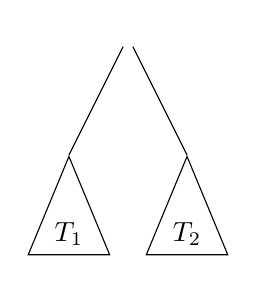
\begin{tikzpicture}
\usetikzlibrary{shapes.geometric}
\node {} [child anchor = apex]
child {node[draw, thin, isosceles triangle, anchor = apex, shape border rotate = 90]{$T_1$}}
child {node[draw, thin, isosceles triangle, anchor = apex, shape border rotate = 90]{$T_2$}};
\end{tikzpicture}

  \caption{Constructing a tree from subtrees}
  \label{fig:BinTreeConstruction}
\end{figure}
Also in addition to drawing pictures of binary trees, we can use a linear notation (something that  can we written 
in the midst of prose). 
If $T_1$ and $T_2$ are simple binary trees, we may denote the tree constructed by grafting $T_1$ on the left and $T_2$ on the right
as $(T_1\wedge T_2)$ (as in Figure \ref{fig:BinTreeConstruction}. Thus we define simple binary trees, and two operations
on them, as follows.

\begin{defn}
\emph{Simple binary trees} are defined inductively by
\[T \defeq \bullet \,\mid\, (T_1\wedge T_2)\]
The \emph{size} of a simple binary tree a natural number defined by the equations
\begin{align*}
  \sz(\bullet) &\defeq 0\\
  \sz(T_1\wedge T_2) &\defeq 1 + \sz(T_1) + \sz(T_2)
\end{align*}
The \emph{height} of a simply binary tree a natural number is defined
by the equations
\begin{align*}
  \hght(\bullet) &\defeq 0\\
  \hght(T_1\wedge T_2) &\defeq 1 + \max(\hght(T_1),\hght(T_2))
\end{align*}
where $\max(m,n)$ is the larger of the two numbers.
\end{defn}

These definitions suggest a relation between the size and height of a tree.
\ipadbreak

\begin{lemma}
For any simple binary tree $T$,  \[\hght(T)\leq \sz(T) < 2^{\hght(T)}.\]

\begin{proof}
To prove this by \emph{structural induction}, we must prove it for the basis ($\bullet$)
and that if it is true for some $T_1$ and $T_2$, then it is true for $(T_1\wedge T_2)$.
\begin{itemize}
\item{}[Basis] $\hght(\bullet) = 0$, $\sz(\bullet) = 0$ 
and $2^{\hght(\bullet)} = 1$. So the claim is true for $\bullet$.
\item{}[Inductive Hypothesis] Suppose the inequalities holds for some $T_1$ and $T_2$.
\item{}[Inductive Step] We must prove the two inequalities for $T= (T_1\wedge T_2)$.
Without loss of generality, assume that $\hght(T_1)\leq \hght(T_2)$. That is, if 
this is not so, then we may swap $T_1$ for $T_2$ in the following. 
\begin{align*}
\hght(T) &= 1 + \max(\hght(T_1),\hght(T_2)) &&\text{[Definition of $\hght$]}\\
         &\leq 1 + \hght(T_1) + \hght(T_2)  &&\text{[Arithmetic]}\\
         &\leq  1 + \sz(T_1) + \sz(T_2) &&\text{[Inductive Hypothesis]}\\
         &= \sz(T) &&\text{[Definition of $\sz$]}
       \end{align*}
And
\begin{align*}
\sz(T) &= 1 +\sz(T_1) + \sz(T_2)&&\text{[Definition of $\sz$]}\\
       &\leq 1 + 2^{\hght(T_1)} - 1) + (2^{\hght(T_2)} - 1)&&\text{[Inductive Hypothesis]}\\
       &\leq 2\cdot 2^{\hght(T_2)} - 1&&\text{[Assumption that $\hght(T_1)\leq \hght(T_2)$]}\\
       &= 2^{\hght(T_2)+1} - 1 &&\text{[Arithmetic]}\\
       &= 2^{\hght(T)} - 1 &&\text{[Definition of $\hght$]}
     \end{align*}
So $\sz(T) < 2^{\hght(T)}$
   \end{itemize}
 \end{proof}  
\end{lemma}

\ipadbreak

\begin{exercises}
  \item Calculate the height and size of the following simple binary trees.
    \begin{enumerate}
    \item $(\bullet\wedge\bullet)$
    \item $(\bullet\wedge (\bullet\wedge\bullet))$
    \item $((\bullet\wedge\bullet)\wedge(\bullet\wedge(\bullet\wedge\bullet)))$
    \item $((\bullet\wedge(\bullet\wedge\bullet))\wedge ((\bullet\wedge\bullet)\wedge(\bullet\wedge(\bullet\wedge\bullet))))$
    \end{enumerate}
   \item Draw diagrams (similar to those in Figure \ref{fig:BinTree}) for the following
   simple binary trees.
   \begin{enumerate}
   \item $((\bullet \wedge \bullet)\wedge(\bullet\wedge\bullet))$
   \item $(((\bullet\wedge\bullet)\wedge\bullet)\wedge ((\bullet\wedge\bullet)\wedge(\bullet\wedge(\bullet\wedge\bullet))))$
   \end{enumerate}
   \item For each of the following diagrams, write the expression using $\bullet$ and $\wedge$
    defining the same tree.
\begin{multicols}{2}
    \begin{enumerate}
    \item 
\begin{tikzpicture}
\node {}
child {node {$\bullet$}}
child {node  {}
       child {node {$\bullet$}}
       child {node {$\bullet$}}
      };
\end{tikzpicture}

 \item 

\begin{tikzpicture}
[level/.style={sibling distance = 2cm/#1, level distance = 1.5cm}]
\node {}
child {node  {}
       child {node {$\bullet$}}
       child {node {$\bullet$}}
      }
child {node  {}
       child {node {$\bullet$}}
       child {node {$\bullet$}}
      };
\end{tikzpicture}

\item

\begin{tikzpicture}
\node {}
child {node  {}
       child {node {} 
              child {node {$\bullet$}}
              child {node {$\bullet$}}}
       child {node {$\bullet$}}
      }
child {node  {$\bullet$}};
\end{tikzpicture}

    \end{enumerate}
  \end{multicols}
\end{exercises}


\begin{exercise}
\newcommand{\unit}{\mathord{\textbf{u}}}
\newcommand{\B}{\mathord{\textbf{B}}}
\newcommand{\C}{\mathord{\textbf{C}}}
\newcommand{\denotation}{\mathord{\textsf{val}}}

A \emph{widget} is defined inductively by
\[M \defeq \unit \mid M\B \,\mid\, M\C\]

For two widgets $M$ and $N$, their
\emph{merge} is a widget, denoted by $M\oplus N$, defined by
\begin{align*}
\unit \oplus \unit &\defeq \unit\B\\
\unit \oplus N\B &\defeq N\C\\
\unit \oplus N\C &\defeq (\unit \oplus N)\B\\ 
M\B \oplus \unit &\defeq M\C\\
M\B \oplus N\B &\defeq (M\oplus N)\B\\
M\B \oplus N\C &\defeq (M\oplus N)\C\\
M\C \oplus \unit &\defeq  (M\oplus \unit)\B\\
M\C \oplus N\B&\defeq (M\oplus N)\C\\
M\C \oplus N\C&\defeq ((M\oplus N) \oplus \unit)\B
\end{align*} 

For a widget $M$, its \emph{value} is a natural number, denoted by
$\llbracket M\rrbracket$, defined by
\begin{align*}
  \llbracket\unit\rrbracket &\defeq 1\\
  \llbracket M\B\rrbracket &\defeq 2\cdot \llbracket M\rrbracket\\
  \llbracket M\C\rrbracket &\defeq 2\cdot \llbracket M\rrbracket + 1
\end{align*}

Show that $\llbracket M\rrbracket + \llbracket N\rrbracket = \llbracket M\oplus N\rrbracket$ for any two
widgets $M$ and $N$.
\end{exercise}
}
%%% Local Variables: 
%%% mode: latex
%%% TeX-master: "MainText"
%%% End: 
